\documentclass[10pt,a4paper]{article}
\usepackage[margin=2.1cm]{geometry}
\usepackage{newtxtext,newtxmath}
\usepackage{graphicx,booktabs,amsmath,xcolor,float,caption,tabularx,siunitx}
\usepackage{tikz}
\usetikzlibrary{arrows.meta,positioning,fit}
\usepackage[hidelinks]{hyperref}
\captionsetup{font=small,labelfont=bf}
\graphicspath{{figures/}{../paper/figures/}}
% generated by scripts/pcb_fab_numbers.py
\newcommand{\QFET}{32.5}
\newcommand{\QCH}{65}
\newcommand{\CissTwenty}{144}
\newcommand{\CdecRatio}{139}
\newcommand{\Ion}{3.1}
\newcommand{\Ioff}{6.5}
\newcommand{\RgFet}{2.0}
\newcommand{\RoffFet}{0.5}
\newcommand{\IoffNoDiodeR}{9.1}
\newcommand{\Vldo}{6.29}
\newcommand{\IgFifty}{3.2}
\newcommand{\ItotFifty}{7.6}
\newcommand{\PgateFifty}{20}
\newcommand{\PldoFifty}{13}
\newcommand{\PchFifty}{61}
\newcommand{\IgHundred}{6.5}
\newcommand{\ItotHundred}{10.8}
\newcommand{\PgateHundred}{41}
\newcommand{\PldoHundred}{19}
\newcommand{\PchHundred}{87}
\newcommand{\Ish}{2.3}
\newcommand{\RPad}{5.3}
\newcommand{\THSrise}{6}
\newcommand{\TjHS}{57}
\newcommand{\PHS}{7.6}
\newcommand{\TjHSWorst}{59}
\newcommand{\BoardW}{42.1}
\newcommand{\BoardH}{85.5}
\newcommand{\NFoot}{134}
\newcommand{\NVia}{235}
\newcommand{\NTrack}{336}
\newcommand{\SpDcpHsInner}{0.65}
\newcommand{\SpDcpHsOuter}{0.20}
\newcommand{\SpDcpLsInner}{1.07}
\newcommand{\SpDcpLsOuter}{0.70}
\newcommand{\SpHsLsInner}{0.38}
\newcommand{\SpHsLsOuter}{0.20}
\newcommand{\SpHsPriInner}{1.08}
\newcommand{\SpHsPriOuter}{1.37}
\newcommand{\SpLsPriInner}{0.75}
\newcommand{\SpLsPriOuter}{1.50}

% generated by simulation/bb_q3d/busbar_post.py (1 MHz AC, DC)
\newcommand{\BusLAcLegOne}{41.12}
\newcommand{\BusRAcLegOne}{4.984}
\newcommand{\BusLAcLegTwo}{41.28}
\newcommand{\BusRAcLegTwo}{4.855}
\newcommand{\BusLAcLegThree}{41.35}
\newcommand{\BusRAcLegThree}{4.772}
\newcommand{\BusLAcAB}{3.35}
\newcommand{\BusLAcAC}{4.37}
\newcommand{\BusRAcAB}{1.757}
\newcommand{\BusLDcLegOne}{85.57}
\newcommand{\BusRDcLegOne}{0.108}
\newcommand{\BusLDcLegTwo}{83.70}
\newcommand{\BusRDcLegTwo}{0.119}
\newcommand{\BusLDcLegThree}{83.05}
\newcommand{\BusRDcLegThree}{0.130}
\newcommand{\BusLDcAB}{8.20}
\newcommand{\BusLDcAC}{12.38}
\newcommand{\BusRDcAB}{0.070}

% generated by simulation/bb_q3d/cs_post.py
\newcommand{\LcsKel}{0.030}
\newcommand{\LgateCs}{1.71}
\newcommand{\MgateOther}{0.010}
\newcommand{\MgateGate}{0.46}
\newcommand{\LcsNoK}{0.061}
\newcommand{\LgateNoK}{1.46}

\definecolor{box}{rgb}{0.93,0.95,0.98}
\definecolor{hs}{rgb}{0.80,0.25,0.20}
\definecolor{ls}{rgb}{0.20,0.40,0.75}
\definecolor{pri}{rgb}{0.25,0.55,0.30}

\title{\textbf{SPB Leg Building Block, Rev A: Fabrication Board}\\[2pt]
\large Gate driver, isolated supplies, DC link, parasitics, connectors and fabrication data}
\author{Enes Ayaz, KTH --- design note for the 2\,$\times$\,EPC2361 per switch building block}
\date{9 October 2026}

\begin{document}
\maketitle

\noindent\colorbox{box}{\parbox{\dimexpr\linewidth-2\fboxsep}{\small
\textbf{Summary.}
\begin{itemize}\itemsep1pt
\item One half-bridge leg (two mirrored commutation cells, 2\,$\times$\,EPC2361 per switch) on a 4-layer, 2\,oz board of 42\,$\times$\,85.4\,mm with DC terminals at one end, the AC terminals directly below the switch nodes, the gate supplies and the lab header on the tab. The layout is generated by \texttt{scripts/make\_kicad\_bb\_fab.py}; DRC: 0 violations, 0 unconnected pads. The wired KiCad schematic (\texttt{spb-bb-fab.kicad\_sch}) has the same netlist as the board (checked net by net), and every part has a 3D model.
\item \textbf{Double-pulse test:} probe landings (tip + spring ground at 2.5 and 5.0\,mm) for $V_\mathrm{DS}$, $V_\mathrm{GS}$ and the source-inductance voltage $v_\mathrm{KS}$ of both low-side transistors and $V_\mathrm{GS}$ of both high-side transistors, placed beside the cells without touching the commutation loop. Bring-up landings and LEDs for the 12\,V input, both isolated module outputs, both regulator outputs and the DC link; PWM pull-downs and a DC-link bleeder.
\item \textbf{Load test cooling:} Fischer LAM 4 K 50 12 fan heatsink (0.65\,K/W, 12\,V fan from J7) on an aluminium spreader with pedestals and 0.4\,mm insulating gap pads, held by four M2.5 screws beside the cells: $T_j\approx$\,\TjHS\,$^\circ$C at the rated point and 40\,$^\circ$C ambient.
\item \textbf{Gate drive:} one 2EDF7275K for both switches, two isolated supplies (one per channel), centre star per switch with Kelvin returns. Separate turn-on and turn-off paths per channel: $R_\mathrm{ON}$ in parallel with a Schottky diode in series with $R_\mathrm{OFF}$, then $R_{G,i}$ per transistor. Default $R_\mathrm{ON}=0.75\,\Omega$, $R_\mathrm{OFF}=0\,\Omega$, $R_{G,i}=0.5\,\Omega$: \RgFet\,$\Omega$ (on) and \RoffFet\,$\Omega$ plus diode (off) external per transistor. Split rail $+5.05/-1.24$\,V from MGN1S1208MC\,$\rightarrow$\,TPS7A4901 (\Vldo\,V)\,$\rightarrow$\,TLV431. A 10\,k$\Omega$ pull-down from each gate star to its Kelvin source holds both gates off when the driver output side is unpowered. Peak gate current \Ion\,A (on) / \Ioff\,A (off) per channel, below the 4/8\,A driver rating.
\item \textbf{Gate loops in the corridor:} the high-side trunk runs on L3 with its Kelvin return stacked directly below on L4; the low-side star is on L1 with the Kelvin collector on L2. Both Kelvin collectors join on the symmetry line, so the two transistors of a switch see identical gate loops.
\item \textbf{DC link:} 2\,$\times$\,6\,$\times$\,1\,\textmu F 0805 at the drains plus 24\,$\times$\,10\,\textmu F 1210 bank, unchanged from the paper design (Table~\ref{tab:caps}).
\item \textbf{Before ordering:} Q3D re-extraction of this routed copper (26 of 168 power vias were removed for clearance and the 0805 pitch went from 1.4 to 1.6\,mm), and an isolation review for the 1200\,V stack (the 2EDF7275K is a functional-isolation part). The Q3D model of the routed copper is prepared (\texttt{simulation/bb\_q3d/run\_bb\_q3d\_fab.cmd}) and runs when the KTH licence server is reachable. Datasheet checks are done (Section~\ref{sec:dscheck}); they replaced the LP2951 by the TPS7A4901.
\end{itemize}}}

\section{Board overview and stack-up}
Fig.~\ref{fig:layers} shows the four copper layers. The board is 4\,mm wider on each side than the power copper: the outer strips carry the heatsink holes, the probe landings and the bring-up landings and LEDs. From top to bottom: the DC terminals J1/J2 (DC$+$, DC$-$), the three MLCC bank rows, the local 0805 capacitors, the two mirrored cells with the high-side (row at $y=4.9$\,mm) and low-side (row at $y=9.2$\,mm) transistors, the driver in the 9\,mm corridor between the cells, the two AC terminals J3/J4 directly below the switch nodes, the two gate-supply chains, the two isolated DC/DC modules and, at the bottom, the primary side with the lab header J5.

\begin{figure}[H]
\centering
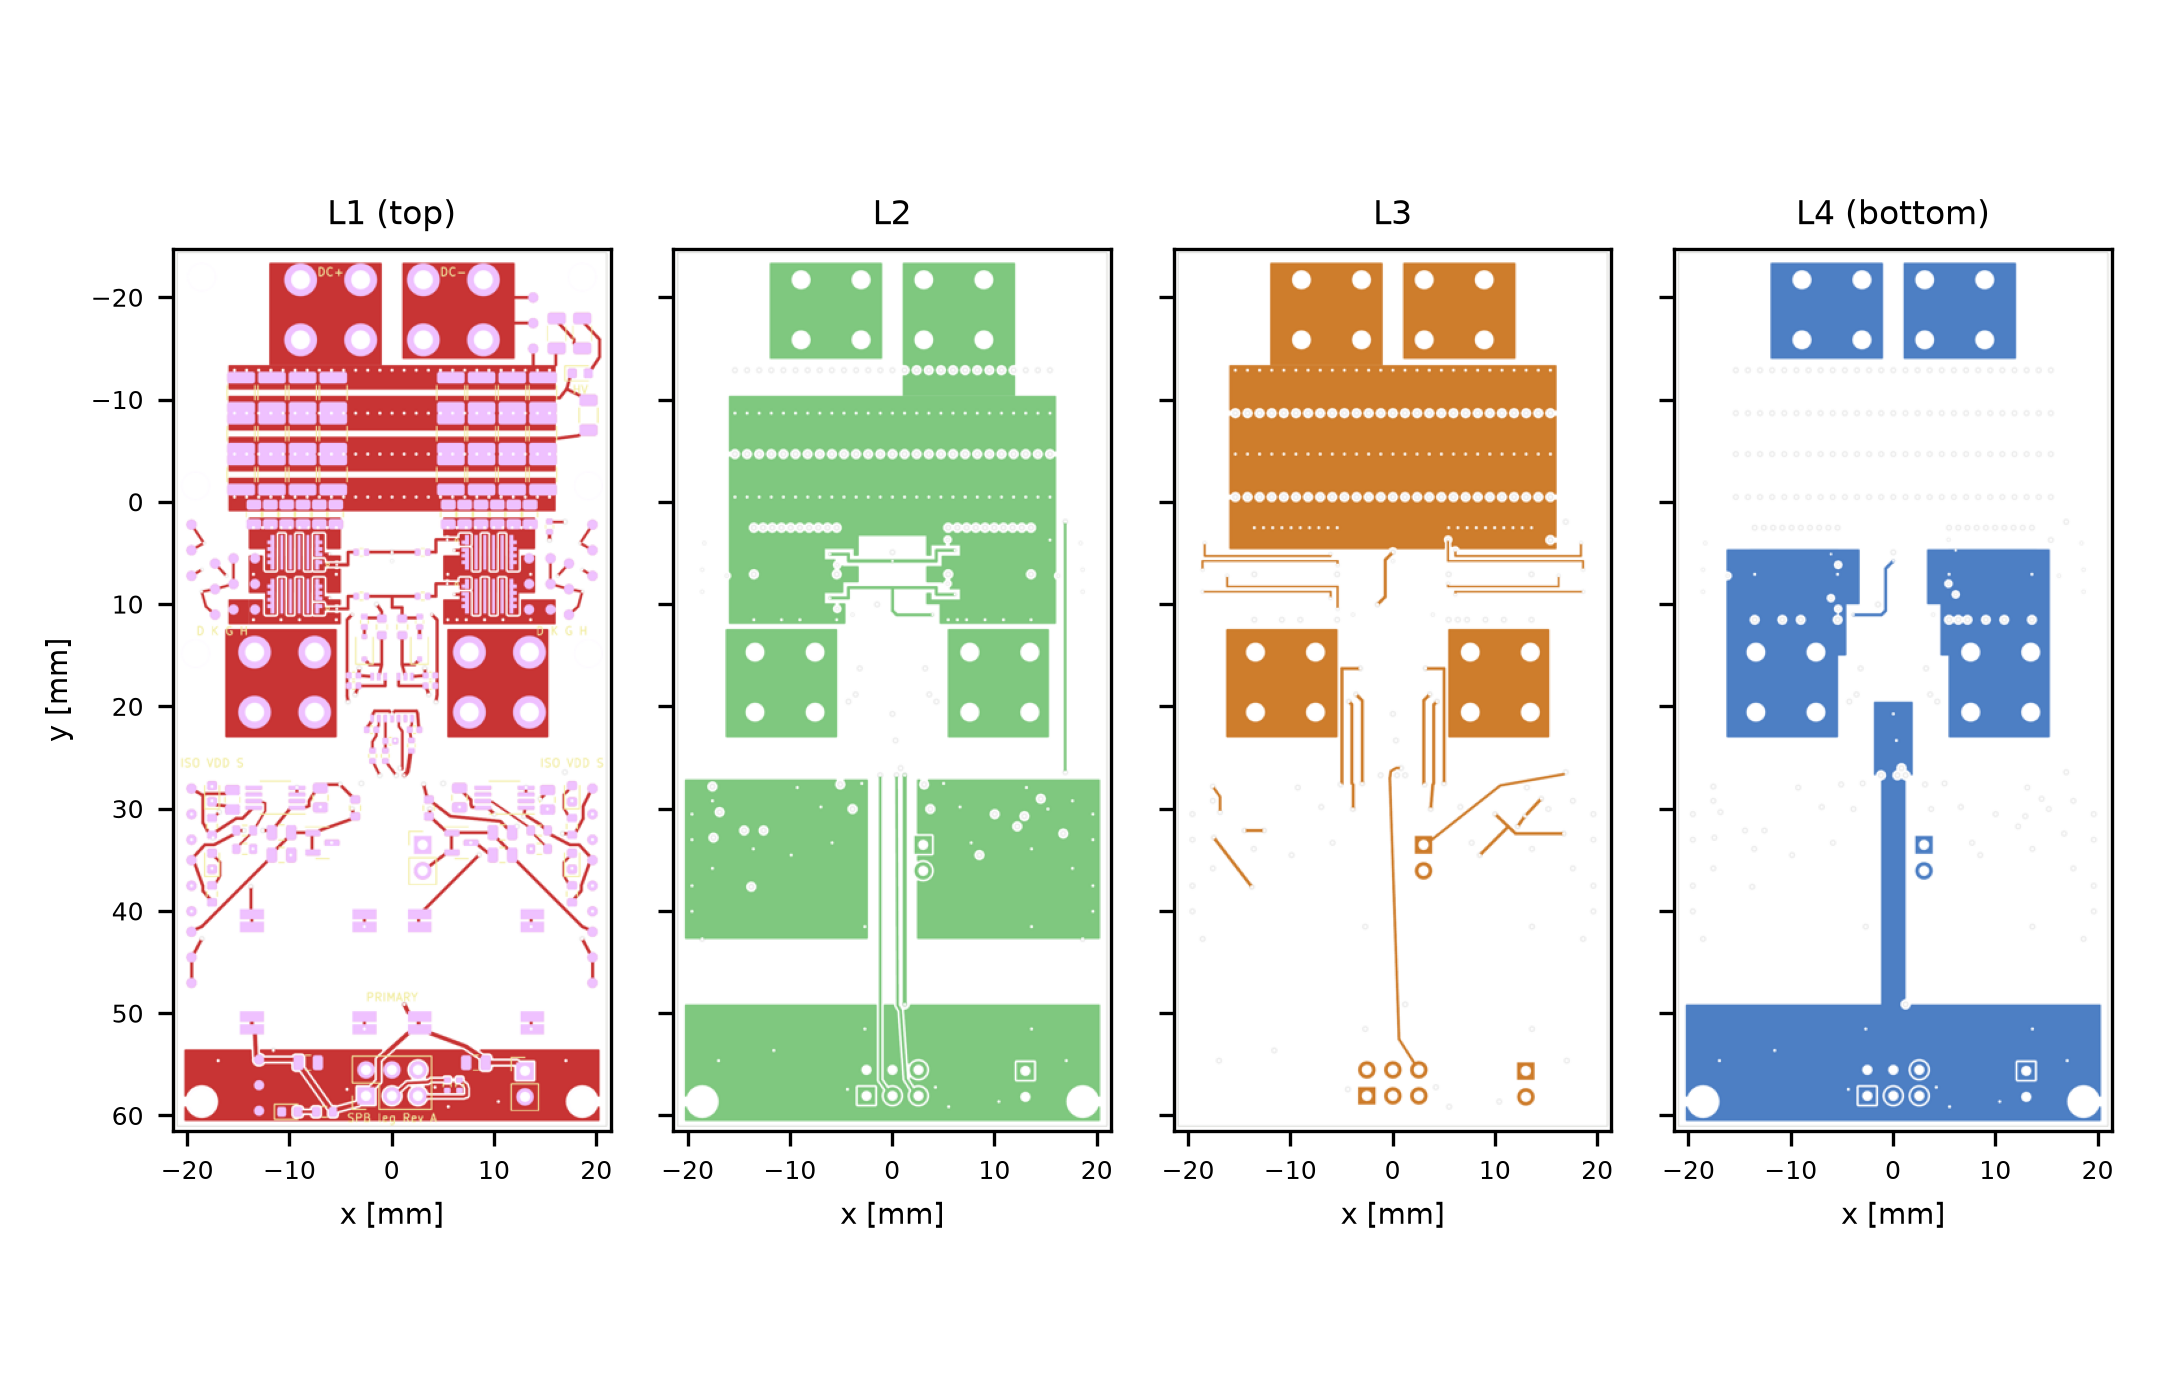
\includegraphics[width=\textwidth]{fig_layers.png}
\caption{Copper layers of the Rev A board (top view on all layers). Red: L1, green: L2 (DC$-$ return plane under the cells, VEE pours under the supply chains, GNDI at the bottom), orange: L3 (DC$+$ plane under the strips and the bank, supply columns), blue: L4 (switch-node plane, GNDI channel and bottom pour).}
\label{fig:layers}
\end{figure}

\begin{table}[H]
\centering\small
\caption{Stack-up and design rules}
\label{tab:stack}
\begin{tabular}{@{}llp{8.2cm}@{}}
\toprule
Item & Value & Use \\
\midrule
L1 (top), 70\,\textmu m & signal / power & FET and capacitor pads, strips, gate stars, all components \\
Prepreg L1--L2 & 0.1\,mm & vertical commutation loop (sets $L_\mathrm{loop}$) \\
L2, 70\,\textmu m & DC$-$ plane & loop return, Kelvin collectors in narrow keepouts, VEE pours on the tab \\
Core L2--L3 & $\approx$\,1.1\,mm & 1.6\,mm total, symmetric build \\
L3, 70\,\textmu m & DC$+$ plane & feed to the cells; HS gate trunk and supply columns in the corridor \\
Prepreg L3--L4 & 0.1\,mm & HS gate trunk (L3) over its Kelvin return (L4) \\
L4 (bottom), 70\,\textmu m & AC plane & switch node to J3/J4; HS Kelvin return under the trunk; GNDI \\
\midrule
Min. track / clearance & 0.15 / 0.15\,mm & signal; power zones 0.2\,mm clearance \\
Vias & 0.6/0.3\,mm (power, signal), 0.45/0.25\,mm (Kelvin) & no via-in-pad, standard process \\
Finish, mask & ENIG, green LPI both sides & mask is the insulation for the 0.2\,mm power gaps \\
\bottomrule
\end{tabular}
\end{table}

The power-copper gaps of 0.2\,mm between DC$+$, DC$-$ and AC on L1 rely on the solder mask: IPC-2221B requires 0.13\,mm for 51--100\,V on coated external conductors (B4) and 0.1\,mm on internal layers (B1), but 0.6\,mm without coating (B2). The board therefore must not be used with exposed copper in the power area (no mask openings other than the pads).

\section{Power transistors}
\begin{table}[H]
\centering\small
\caption{EPC2361 (datasheet, typical at 25\,$^\circ$C unless noted)}
\label{tab:fet}
\begin{tabular}{@{}lll@{}}
\toprule
Parameter & Value & Note \\
\midrule
$V_\mathrm{DS}$ / $V_\mathrm{DS(tr)}$ & 100\,V / 120\,V & 75\,V submodule voltage (75\,\% utilisation) \\
$R_\mathrm{DS(on)}$ & 0.75\,m$\Omega$ (1.0 max) & $V_\mathrm{GS}=5$\,V, 50\,A \\
$I_\mathrm{D}$ cont. / pulsed & 133\,A / 697\,A & \\
$V_\mathrm{GS}$ range & $-4$ \dots\ $+6$\,V & split rail $+5.05/-1.24$\,V \\
$V_\mathrm{GS(th)}$ & 0.8 / 1.1 / 2.5\,V (min/typ/max) & bump $\approx$\,1.06\,V at 0\,V off, removed at $-1.24$\,V \\
$C_\mathrm{iss}$ / $C_\mathrm{oss}$ / $C_\mathrm{rss}$ & 3599 / 1019 / 13\,pF & $V_\mathrm{DS}=50$\,V \\
$Q_\mathrm{G}$ / $Q_\mathrm{GS}$ / $Q_\mathrm{GD}$ & 28 / 8.5 / 3.8\,nC & $V_\mathrm{DS}=50$\,V, 50\,A \\
$Q_\mathrm{OSS}$, $Q_\mathrm{RR}$ & 90\,nC, 0 & \\
$R_\mathrm{G}$ internal & 0.4\,$\Omega$ & \\
$R_{\theta\mathrm{JC}}$ (top) / $R_{\theta\mathrm{JB}}$ & 0.2 / 1.5\,K/W & top-side cooling through TIM to the cold plate \\
Package & 3\,$\times$\,5\,mm, 7 stripes, 0.85\,mm pitch & pin 1 gate, 2/4/6 source, 3/5/7 drain \\
\bottomrule
\end{tabular}
\end{table}

The land pattern is the solder-mask-defined EPC pattern (\texttt{hardware/epc2361-cell}). The drain stripes connect to the DC$+$ copper at one end of the package and the source stripes to the AC (high side) or DC$-$ (low side) copper at the other end, as a comb on L1. The power vias are kept 0.3\,mm outside the stripe ends (rows moved from 2.8 to 2.5\,mm and from 11.1 to 11.5\,mm). Between the high-side source and low-side drain stripes only 0.7\,mm remains, which is too narrow for a via; the AC vias there were removed, and the switch node reaches L4 through the vias beside the packages. The package is chiral, so the left cell is rotated by 180$^\circ$. The gate pads then lie at $y = y_\mathrm{row}\pm 1.23$\,mm, and the star on the symmetry line gives equal branch lengths.

\section{Gate driver}
\subsection{Circuit}
\begin{figure}[H]
\centering
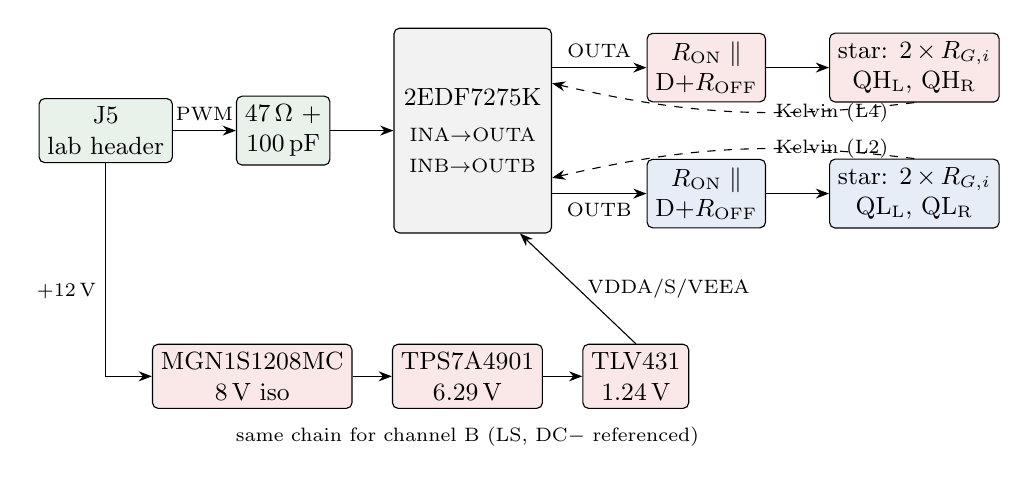
\begin{tikzpicture}[font=\small,>=Stealth,
  blk/.style={draw,rounded corners=2pt,minimum height=8mm,align=center,inner sep=3pt},
  lab/.style={font=\scriptsize,align=center}]
\node[blk,fill=pri!12] (j5) {J5\\lab header};
\node[blk,fill=pri!12,right=8mm of j5] (rc) {47\,$\Omega$ +\\100\,pF};
\node[blk,fill=black!5,right=8mm of rc,minimum height=26mm,minimum width=20mm] (drv) {2EDF7275K\\[2pt]\scriptsize INA$\rightarrow$OUTA\\\scriptsize INB$\rightarrow$OUTB};
\node[blk,fill=hs!12,right=12mm of drv,yshift=8mm] (ra) {$R_\mathrm{ON}\parallel$\\D+$R_\mathrm{OFF}$};
\node[blk,fill=ls!12,right=12mm of drv,yshift=-8mm] (rb) {$R_\mathrm{ON}\parallel$\\D+$R_\mathrm{OFF}$};
\node[blk,fill=hs!12,right=8mm of ra] (sa) {star: 2\,$\times$\,$R_{G,i}$\\QH$_\mathrm{L}$, QH$_\mathrm{R}$};
\node[blk,fill=ls!12,right=8mm of rb] (sb) {star: 2\,$\times$\,$R_{G,i}$\\QL$_\mathrm{L}$, QL$_\mathrm{R}$};
\draw[->] (j5) -- node[lab,above]{PWM} (rc);
\draw[->] (rc) -- (drv);
\draw[->] (drv.east|-ra) -- node[lab,above]{OUTA} (ra);
\draw[->] (drv.east|-rb) -- node[lab,below]{OUTB} (rb);
\draw[->] (ra) -- (sa); \draw[->] (rb) -- (sb);
\draw[dashed,->] (sa.south) to[bend left=10] node[lab,right,pos=0.4]{Kelvin (L4)} ([yshift=-2mm]drv.east|-ra);
\draw[dashed,->] (sb.north) to[bend right=10] node[lab,right,pos=0.4]{Kelvin (L2)} ([yshift=2mm]drv.east|-rb);
\node[blk,fill=hs!12,below=14mm of drv,xshift=-28mm] (pa) {MGN1S1208MC\\8\,V iso};
\node[blk,fill=hs!12,right=5mm of pa] (la) {TPS7A4901\\6.29\,V};
\node[blk,fill=hs!12,right=5mm of la] (ta) {TLV431\\1.24\,V};
\draw[->] (pa) -- (la); \draw[->] (la) -- (ta);
\draw[->] (ta.north) -- node[lab,right]{VDDA/S/VEEA} ([xshift=6mm]drv.south);
\node[lab,below=1mm of la] {same chain for channel B (LS, DC$-$ referenced)};
\draw[->] (j5.south) |- node[lab,left,pos=0.3]{+12\,V} (pa.west);
\end{tikzpicture}
\caption{Gate-drive circuit of the leg. Colours mark the isolation domains: primary (green, GNDI), high side (red, switch-node referenced), low side (blue, DC$-$ referenced).}
\label{fig:gd}
\end{figure}

The driver's input side runs from the 12\,V lab supply in SLDO mode (SLDON to GNDI, $R_\mathrm{VDDI}=3\,\mathrm{k}\Omega$, 22\,nF at VDDI). Each PWM input has a 47\,$\Omega$/100\,pF filter ($\tau=4.7$\,ns) against cable ringing; DISABLE is driven from the header (the driver's internal pull-down keeps it enabled when open). Channel A drives the high side and channel B the low side; dead time is generated by the controller.

\subsection{Gate network: separate turn-on and turn-off paths}
The 2EDF7275K has one output pin per channel, so separate turn-on and turn-off resistances need a steering diode. Each channel has
\[
\text{OUT}\;\rightarrow\;\bigl(R_\mathrm{ON}\;\parallel\;(D + R_\mathrm{OFF})\bigr)\;\rightarrow\;\text{trunk}\;\rightarrow\;\text{star}\;\rightarrow\;R_{G,i}\;\rightarrow\;\text{gate}_i,
\]
with the diode (PMEG3020EJ, SOD323F, cathode toward the driver output) conducting only when the driver pulls the gate down. Because the two transistors of a switch share the channel network, each transistor sees it twice:
\[
R_\mathrm{on,eff}=2R_\mathrm{ON}+R_{G,i},\qquad R_\mathrm{off,eff}=2\bigl(R_\mathrm{ON}\parallel(R_\mathrm{OFF}+r_D)\bigr)+R_{G,i}\;(+\,V_F),
\]
plus $R_\mathrm{G,int}=0.4\,\Omega$ and twice the driver output resistance (0.85\,$\Omega$ pull-up, 0.35\,$\Omega$ pull-down). The default population $R_\mathrm{ON}=0.75\,\Omega$ (0603), $R_\mathrm{OFF}=0\,\Omega$ (0402 jumper), $R_{G,i}=0.5\,\Omega$ (0402) gives \RgFet\,$\Omega$ on and \RoffFet\,$\Omega$ plus the diode off per transistor, i.e. the simulated $R_\mathrm{g,on}/R_\mathrm{g,off}=2/0\,\Omega$ with the 0.5\,$\Omega$ star resistors kept for damping between the paralleled gates. The peak sink current is then \Ioff\,A per channel ($\approx$\,\IoffNoDiodeR\,A if also $R_{G,i}=0$), inside the 8\,A rating; $R_\mathrm{ON}$, $R_\mathrm{OFF}$ and $R_{G,i}$ can be changed independently by population. Below the diode forward voltage ($\approx$\,0.4\,V) the gate is pulled the rest of the way to $-1.24$\,V through $R_\mathrm{ON}$. The networks sit between the low-side star and the driver (Fig.~\ref{fig:corridor}); to make room the driver and the tab moved 3.5\,mm down (board 34\,$\times$\,85.4\,mm).

\begin{table}[H]
\centering\small
\caption{Gate-drive budget per channel (two EPC2361, $V_\mathrm{DD}-V_\mathrm{EE}=6.29$\,V)}
\label{tab:budget}
\begin{tabular}{@{}lrr@{}}
\toprule
 & 50\,kHz & 100\,kHz \\
\midrule
Gate charge per transistor, $Q_\mathrm{G}(5\,\mathrm{V})+C_\mathrm{iss}\cdot1.24\,\mathrm{V}$ & \multicolumn{2}{c}{\QFET\,nC} \\
Gate charge per channel & \multicolumn{2}{c}{\QCH\,nC} \\
Peak gate current, turn-on / turn-off (default population) & \multicolumn{2}{c}{\Ion\,A / \Ioff\,A} \\
Gate supply current $Q_\mathrm{ch}f$ & \IgFifty\,mA & \IgHundred\,mA \\
Gate drive power $Q_\mathrm{ch}\Delta V f$ & \PgateFifty\,mW & \PgateHundred\,mW \\
Total chain current (incl. 2\,mA driver, \Ish\,mA shunt bias) & \ItotFifty\,mA & \ItotHundred\,mA \\
LDO dissipation & \PldoFifty\,mW & \PldoHundred\,mW \\
MGN1 output power (125\,mA, 1\,W rating) & \PchFifty\,mW & \PchHundred\,mW \\
\bottomrule
\end{tabular}
\end{table}

\subsection{Decoupling}
Each half rail of each channel has a 1\,\textmu F/16\,V X7R 0402 directly at the driver (VDD--S and S--VEE), i.e. \CdecRatio\,$\times$ the input capacitance of the two transistors (rule of thumb: $\geq 20\,C_\mathrm{iss}=\CissTwenty$\,nF). A further 4.7\,\textmu F per half rail and 10\,\textmu F VDD--VEE sit at the regulator, 10--12\,mm away on the L3 supply columns, and supply the average current.

\subsection{Gate-loop layout}
\begin{figure}[H]
\centering
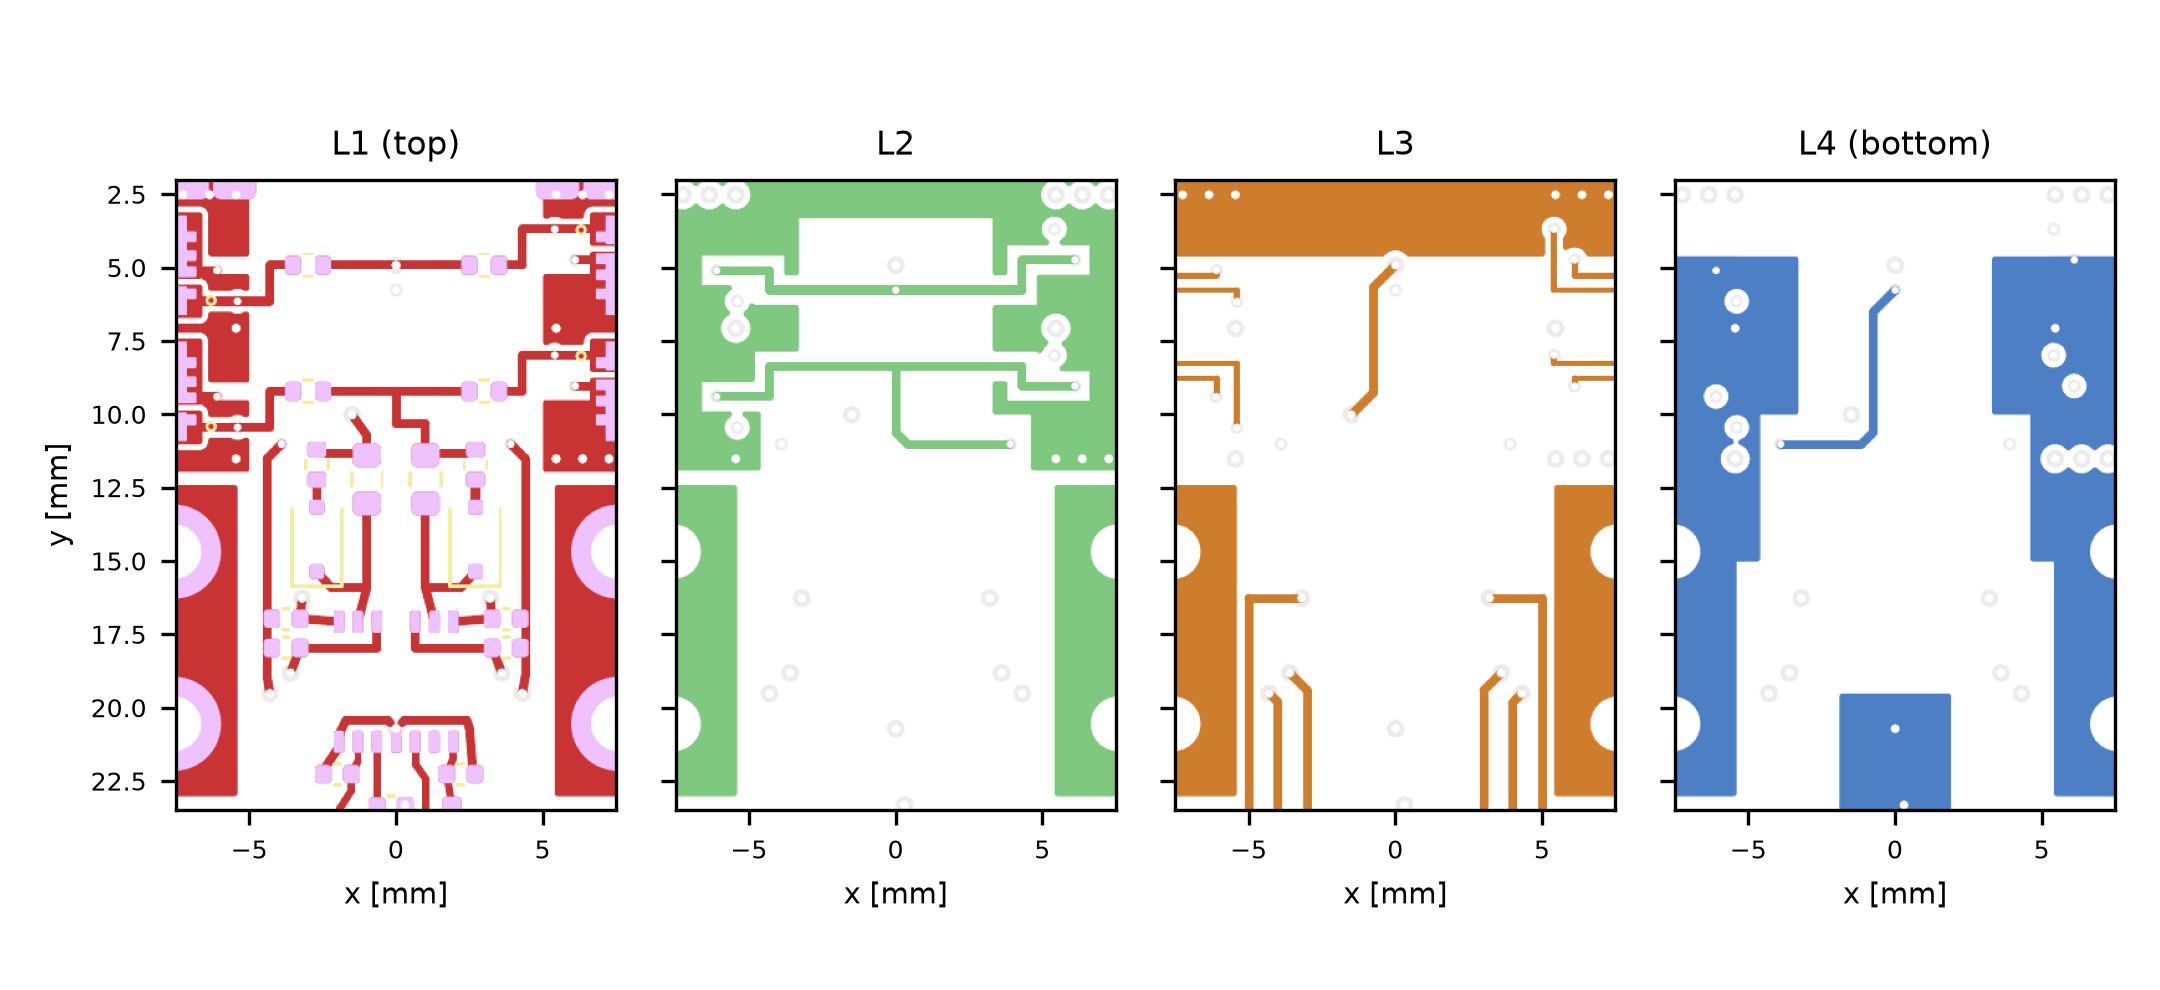
\includegraphics[width=\textwidth]{fig_corridor.png}
\caption{Driver corridor between the cells. L1: high-side star (upper row) and low-side star (lower row), each with two $R_{G,i}$; per channel $R_\mathrm{ON}$ (inner column) and $R_\mathrm{OFF}$ with the diode (outer column) above the 2EDF7275K; local decoupling to the left (A) and right (B) of the driver. L2: Kelvin collectors from the source-pad ends to the symmetry line in narrow keepouts of the DC$-$ plane; the low-side collector continues to the B decoupling. L3: high-side trunk from the star via down the corridor; supply columns of both chains. L4: high-side Kelvin return directly under the L3 trunk inside the corridor keepout of the switch-node plane.}
\label{fig:corridor}
\end{figure}

The extracted gate loop of the paper geometry is \LgateCs\,nH per transistor with a common-source inductance of \LcsKel\,nH (Q3D, Kelvin via at the source pad). The fabrication layout keeps the topology (star on the symmetry line, Kelvin at the source-pad end next to the gate) but lengthens the trunk into the wider corridor. The high-side pair (L3 trunk 0.1\,mm above its L4 return) and the low-side pair (L1 trunk, L2 collector) are broadside-coupled, which keeps the loop area small, but their inductance must be re-extracted.

\section{Isolated gate supplies}
Each channel has its own MGN1S1208MC (12\,V\,$\rightarrow$\,8\,V, 125\,mA, 2.5\,pF isolation capacitance, CMTI $>200$\,kV/\textmu s). Its unregulated 8\,V output feeds a TPS7A4901 low-dropout regulator (TI, 3--35\,V input, 150\,mA, HVSSOP-8 PowerPAD) set by a divider:
\[
V_\mathrm{DD}-V_\mathrm{EE}=1.185\,\mathrm{V}\left(1+\frac{102\,\mathrm{k}\Omega}{23.7\,\mathrm{k}\Omega}\right)=\Vldo\,\mathrm{V}.
\]
A TLV431A between the source node S (cathode and reference) and VEE (anode) holds S at 1.24\,V above VEE; 2.2\,k$\Omega$ from VDD supplies the shunt bias (\Ish\,mA), so that $V_\mathrm{DD}-V_\mathrm{S}=+5.05$\,V and $V_\mathrm{EE}-V_\mathrm{S}=-1.24$\,V. The driver's 4\,V UVLO refers to VDD$-$VEE\,=\,6.29\,V and is not affected. EN is tied to IN, NR/SS is left open ($C_\mathrm{NR}=0$ is allowed), DNC and NC are not connected and the exposed pad goes to VEE. The regulator is stable with ceramic output capacitors $\geq 2.2$\,\textmu F (10\,\textmu F + 4.7\,\textmu F here), needs about 0.3\,V headroom at the load and accepts the light-load rise of the MGN1 output (inputs rated 25\,V).

\subsection{Datasheet checks}\label{sec:dscheck}
\begin{itemize}
\item \textbf{LP2951 replaced.} TI's LP2951 (SLVS582L) is not offered in VSSOP (only SOIC, PDIP, WSON), and the adjustable SOIC part may ship with the legacy chip, which requires 30\,m$\Omega$--5\,$\Omega$ output-capacitor ESR, more than ceramic capacitors provide. The TPS7A4901DGNR in the same 3\,$\times$\,3\,mm footprint size is ceramic-stable; pinout per SBVS121E: 1 OUT, 2 FB, 3 NC, 4 GND, 5 EN, 6 NR/SS, 7 DNC, 8 IN, exposed pad to GND.
\item \textbf{TLV431 (SLVS139Z).} DBZ pinout 1 REF, 2 CATHODE, 3 ANODE, as on the board. Cathode current range 0.1--15\,mA (here $\approx$\,2.3\,mA). With cathode tied to REF the shunt can oscillate between about 0.02 and 0.8\,\textmu F load capacitance at a few mA; the S--VEE node has 4.7\,\textmu F plus 1\,\textmu F ceramic, in the stable region.
\item \textbf{PMEG3020EJ.} Nexperia PMEG3020EJ,115: SOD323F, 30\,V, 2\,A, $I_\mathrm{FSM}$ 9\,A, $C_d\approx$\,60--70\,pF; pin 1 cathode as on the footprint. The 6.5\,A turn-off peaks last nanoseconds.
\end{itemize}

The MGN1 sits with its output pins toward the chain and its input pins toward the primary strip, so that its internal barrier (8.75\,mm between the pin rows) separates the high-voltage and primary sides of the board. The VEE pours on L2 under each chain give the regulator a return plane in its own domain.

\section{DC-link capacitors}
The DC link is unchanged from the paper (Section V there): six 1\,\textmu F 0805 per cell directly at the high-side drains define the commutation loop, and the 24\,$\times$\,10\,\textmu F 1210 bank supplies the ripple charge. The only fabrication change is the 0805 pitch of 1.6\,mm (was 1.4\,mm), so that neighbouring pads keep 0.15\,mm.

\begin{table}[H]
\centering\small
\caption{DC-link capacitors per leg (75\,V, 50\,kHz, rated point)}
\label{tab:caps}
\begin{tabular}{@{}lcc@{}}
\toprule
 & local (per cell) & bank \\
\midrule
Part & TDK C2012X7S2A105K125AB & Murata GRM32EC72A106KE05L \\
Size, dielectric & 0805, X7S, 100\,V & 1210, X7S, 100\,V \\
Number per leg & 2\,$\times$\,6 & 24 (3 rows of 8) \\
$C_\mathrm{nom}$ / $C_\mathrm{eff}$ at 75\,V$^\ast$ & 1\,\textmu F / 0.45\,\textmu F & 10\,\textmu F / 3.0\,\textmu F \\
ESR$^\ast$ / ESL$^\ast$ per part & 6\,m$\Omega$ / 0.48\,nH & 3\,m$\Omega$ / 0.5\,nH \\
Self-resonance & 10.8\,MHz & 4.1\,MHz \\
Ripple current per part & 1.1\,A$_\mathrm{rms}$ & 2.0--2.1\,A$_\mathrm{rms}$ \\
Loss per part & 7.5\,mW & 11.5--13.3\,mW \\
\bottomrule
\multicolumn{3}{@{}l}{\footnotesize $^\ast$assumed; to be confirmed with manufacturer models and impedance measurements}
\end{tabular}
\end{table}

\begin{figure}[H]
\centering
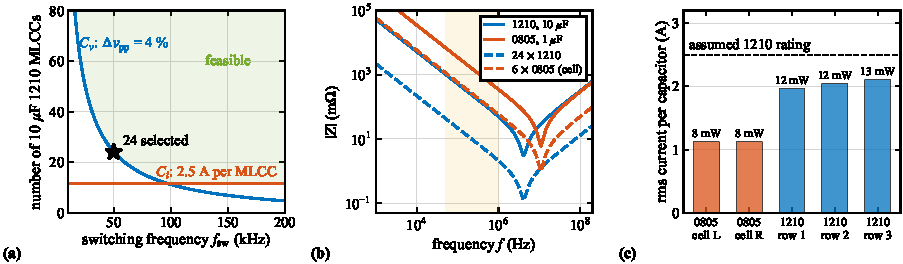
\includegraphics[width=\textwidth]{fig_dclink.pdf}
\caption{DC-link design (from the paper): (a) number of 1210 MLCCs set by voltage ripple and by ripple current, (b) impedance of parts, bank and local group, (c) rms current and loss per capacitor. Total capacitor loss per leg $\approx$\,0.39\,W.}
\end{figure}

\section{Parasitics}
\begin{table}[H]
\centering\small
\caption{Parasitics of the building block and of the cell busbar}
\label{tab:para}
\begin{tabular}{@{}llr@{}}
\toprule
Quantity & Source & Value \\
\midrule
Power-loop inductance per cell & Q3D (paper geometry, 100\,MHz) & 0.374\,nH \\
Gate loop $L_G$ per transistor & Q3D BB\_CS & \LgateCs\,nH \\
Common-source inductance, Kelvin / no Kelvin & Q3D BB\_CS & \LcsKel\,/\,\LcsNoK\,nH \\
Mutual gate loop -- gate loop & Q3D BB\_CS & \MgateGate\,nH \\
ESL per MLCC, 0805 / 1210 & assumed & 0.48 / 0.5\,nH \\
\midrule
Busbar, leg to leg (A--B / A--C), 1\,MHz & Q3D BB\_BUS & \BusLAcAB\,/\,\BusLAcAC\,nH \\
Busbar, leg to leg resistance A--B, 1\,MHz & Q3D BB\_BUS & \BusRAcAB\,m$\Omega$ \\
Busbar, series tab to leg (legs 1/2/3), 1\,MHz & Q3D BB\_BUS & \BusLAcLegOne\,/\,\BusLAcLegTwo\,/\,\BusLAcLegThree\,nH \\
Busbar, series tab to leg, DC & Q3D BB\_BUS & \BusLDcLegOne\,nH, \BusRDcLegOne\,m$\Omega$ \\
\bottomrule
\end{tabular}
\end{table}

The 0.2\,mm gaps, via rows and plane outlines of the fabrication board follow the Q3D geometry, but 26 of the 168 power vias were removed for clearance to the FET stripes and the Kelvin traces, and the via rows were shifted. The 0.374\,nH per cell is therefore a design value until the routed board is re-extracted (\texttt{simulation/bb\_q3d}, import of the KiCad copper).

\textbf{Busbar.} The laminated cell busbar has 3.35\,nH between neighbouring legs, which is what matters for the high-frequency current exchange between the three legs of a submodule (the local MLCCs close the commutation loops). The 41\,nH from the series tab to a leg arise because the DC$+$ and DC$-$ series tabs leave the cell at opposite ends and are not laminated there. This is acceptable for the low-frequency submodule current but should be reduced in the cell assembly by bringing both tabs out at the same end, or by a laminated cell-to-cell interconnect.


\section{Double-pulse test: measurement landings}
For the double-pulse test the low-side switch (Q3 and Q4) is the device under test, the load inductor is connected between DC$+$ (J1) and AC (J3/J4), and Q1/Q2 are held off at $-1.24$\,V. All low-side quantities refer to DC$-$, so ordinary passive probes can be used when the oscilloscope ground is on DC$-$. No measurement part sits in the cells: the landings are bare pads with a tip pad and two spring-ground pads at 2.5 and 5.0\,mm, so both common probe-tip sizes fit without an adapter (Fig.~\ref{fig:landings}).

\begin{figure}[H]
\centering
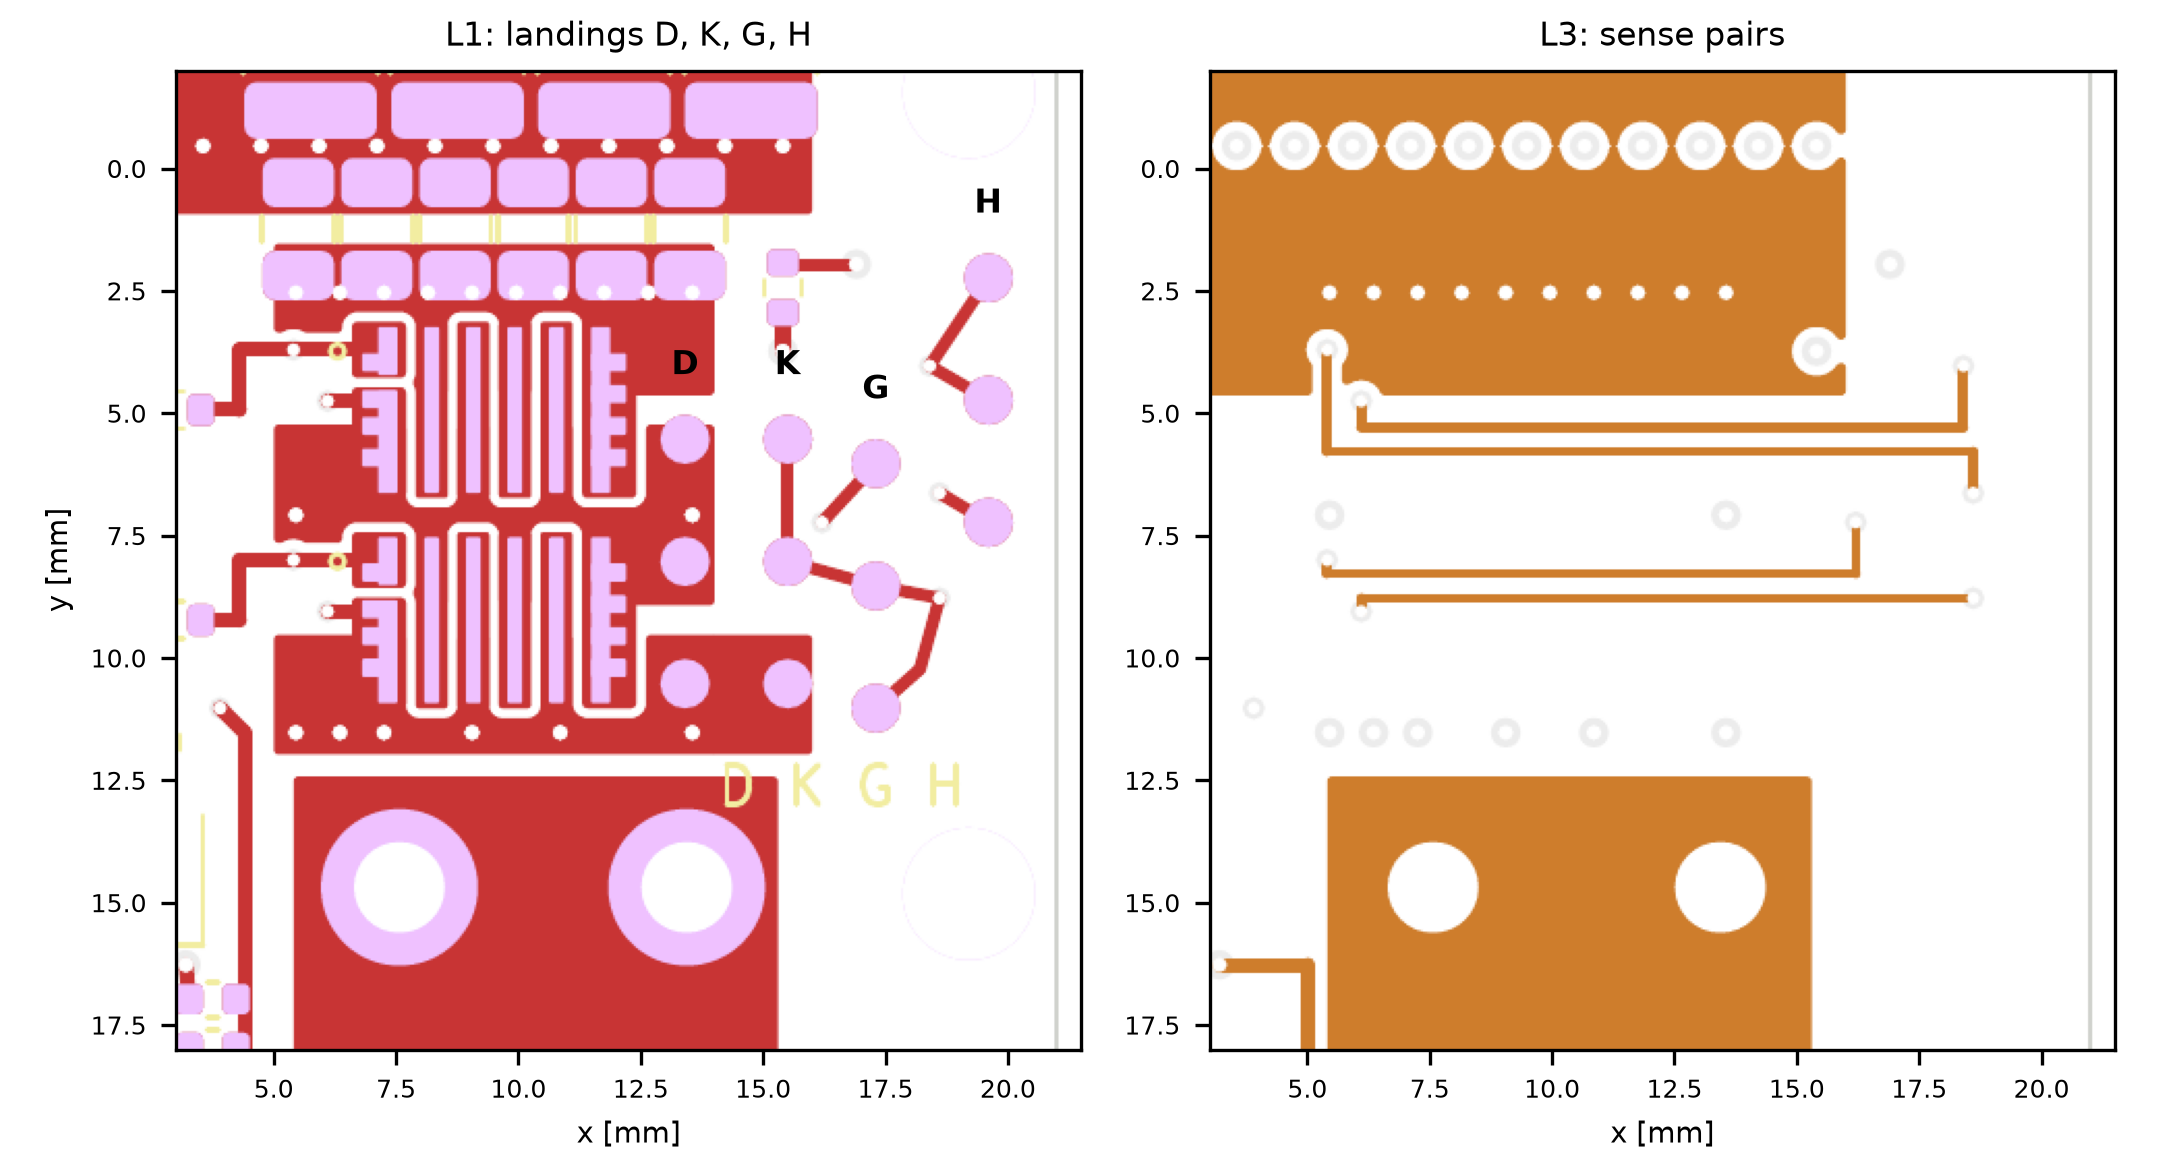
\includegraphics[width=0.95\textwidth]{fig_landings.png}
\caption{Measurement landings at the right cell (the left cell is mirrored). L1: D = $V_\mathrm{DS}$ of Q4 (tips on the switch-node copper next to the package, ground on its source copper), K = $v_\mathrm{KS}$ (tips on the Kelvin sense, ground on the source copper), G = $V_\mathrm{GS}$ of Q4 (tip gate, grounds Kelvin), H = $V_\mathrm{GS}$ of Q2 for an isolated probe. L3: gate and Kelvin sense lines of Q2 and Q4 run as pairs from the gate pad and the Kelvin via to the landings; no current flows in them.}
\label{fig:landings}
\end{figure}

\begin{table}[H]
\centering\small
\caption{Measurement landings (left / right cell)}
\label{tab:landings}
\begin{tabularx}{\textwidth}{@{}llX@{}}
\toprule
Landing & Signal / ground & Use \\
\midrule
TP1 / TP5 (D) & SW / DC$-$ at Q3 / Q4 & $V_\mathrm{DS}$ of each low-side transistor; switching energy with the inductor current \\
TP2 / TP6 (K) & Kelvin sense / source copper & $v_\mathrm{KS}=L_s\,\mathrm{d}i_D/\mathrm{d}t$: per-transistor current change by integration, scaled so that $i_3+i_4=I_L$ \\
TP3 / TP7 (G) & gate / Kelvin of Q3 / Q4 & $V_\mathrm{GS}$ of each low-side transistor (sharing, Miller plateau, bump) \\
TP4 / TP8 (H) & gate / Kelvin of Q1 / Q2 & $V_\mathrm{GS}$ of the high side, isolated probe only (gate bump at the low-side turn-on) \\
TP16 & DC$+$ / DC$-$ & DC-link voltage (outside the loop) \\
\bottomrule
\end{tabularx}
\end{table}

The switched current is measured off the board with a Rogowski coil or a Pearson monitor on the inductor lead. $E_\mathrm{off}=\int v_\mathrm{DS}\,i\,\mathrm{d}t$ uses $i=I_L$; for $E_\mathrm{on}$ the inductor current misses the output-charge current of the high side, which is added as $Q_\mathrm{OSS}V_\mathrm{DC}$ (2\,$\times$\,90\,nC). The voltage and current channels must be deskewed to better than 50\,ps: at 50\,V/ns and 100\,A a 100\,ps skew changes the energy by about 0.75\,\textmu J. With the heatsink mounted the landings beside the cells are covered by the spreader; they are for the double-pulse test without heatsink.

\section{Bring-up landings, indicators and protection}
\begin{table}[H]
\centering\small
\caption{Bring-up landings and LEDs}\label{tab:bringup}
\begin{tabularx}{\textwidth}{@{}llX@{}}
\toprule
Item & Nets & Expected \\
\midrule
TP15, D7 (green) & +12\,V / GNDI & 12\,V input present (LED 2\,mA via 4.7\,k$\Omega$) \\
TP9, D3 / TP12, D5 & ISO$_\mathrm{A,B}$ / VEE & MGN1 output 8--10\,V (unregulated, light load higher); LED via 2.7\,k$\Omega$ \\
TP10, D4 / TP13, D6 & VDD / VEE & 6.29\,V from the TPS7A4901; LED via 1.8\,k$\Omega$ \\
TP11 / TP14 & S / VEE & 1.24\,V (TLV431), i.e. VDD$-$S $=$ 5.05\,V, VEE$-$S $=-1.24$\,V \\
TP16, D8 (red) & DC$+$ / DC$-$ & DC link charged (0.5\,mA via 2\,$\times$\,68\,k$\Omega$); R39 100\,k$\Omega$ bleeder \\
R35, R36 & PWM\_H, PWM\_L & 10\,k$\Omega$ pull-downs: both switches stay off with the header open \\
J7 & +12\,V / GNDI & fan of the heatsink \\
\bottomrule
\end{tabularx}
\end{table}
The driver outputs and the gate stars are probed directly on the resistor pads (R5/R7: OUT, R1--R4: gates) during bring-up without DC-link voltage. Landings in the gate-supply domains are referenced to the switch node (A) or DC$-$ (B) and must only be probed with the DC link discharged or with an isolated probe.

\section{Cooling for the load test}
EPC2361 is cooled through its top, which is at source potential, so the thermal interface must insulate. Following the EPC thermal concept, the heatsink is screwed to the board around the transistors (Fig.~\ref{fig:heatsink}): a machined aluminium spreader (42\,$\times$\,14\,$\times$\,3\,mm with four ears for M2.5 screws in H5--H8) carries a 0.6\,mm pedestal over each cell, so that the 1.25\,mm high 0805 capacitors beside the transistors are cleared while the gap pad stays thin; a fan heatsink sits on the spreader with thermal grease.

\begin{figure}[H]
\centering
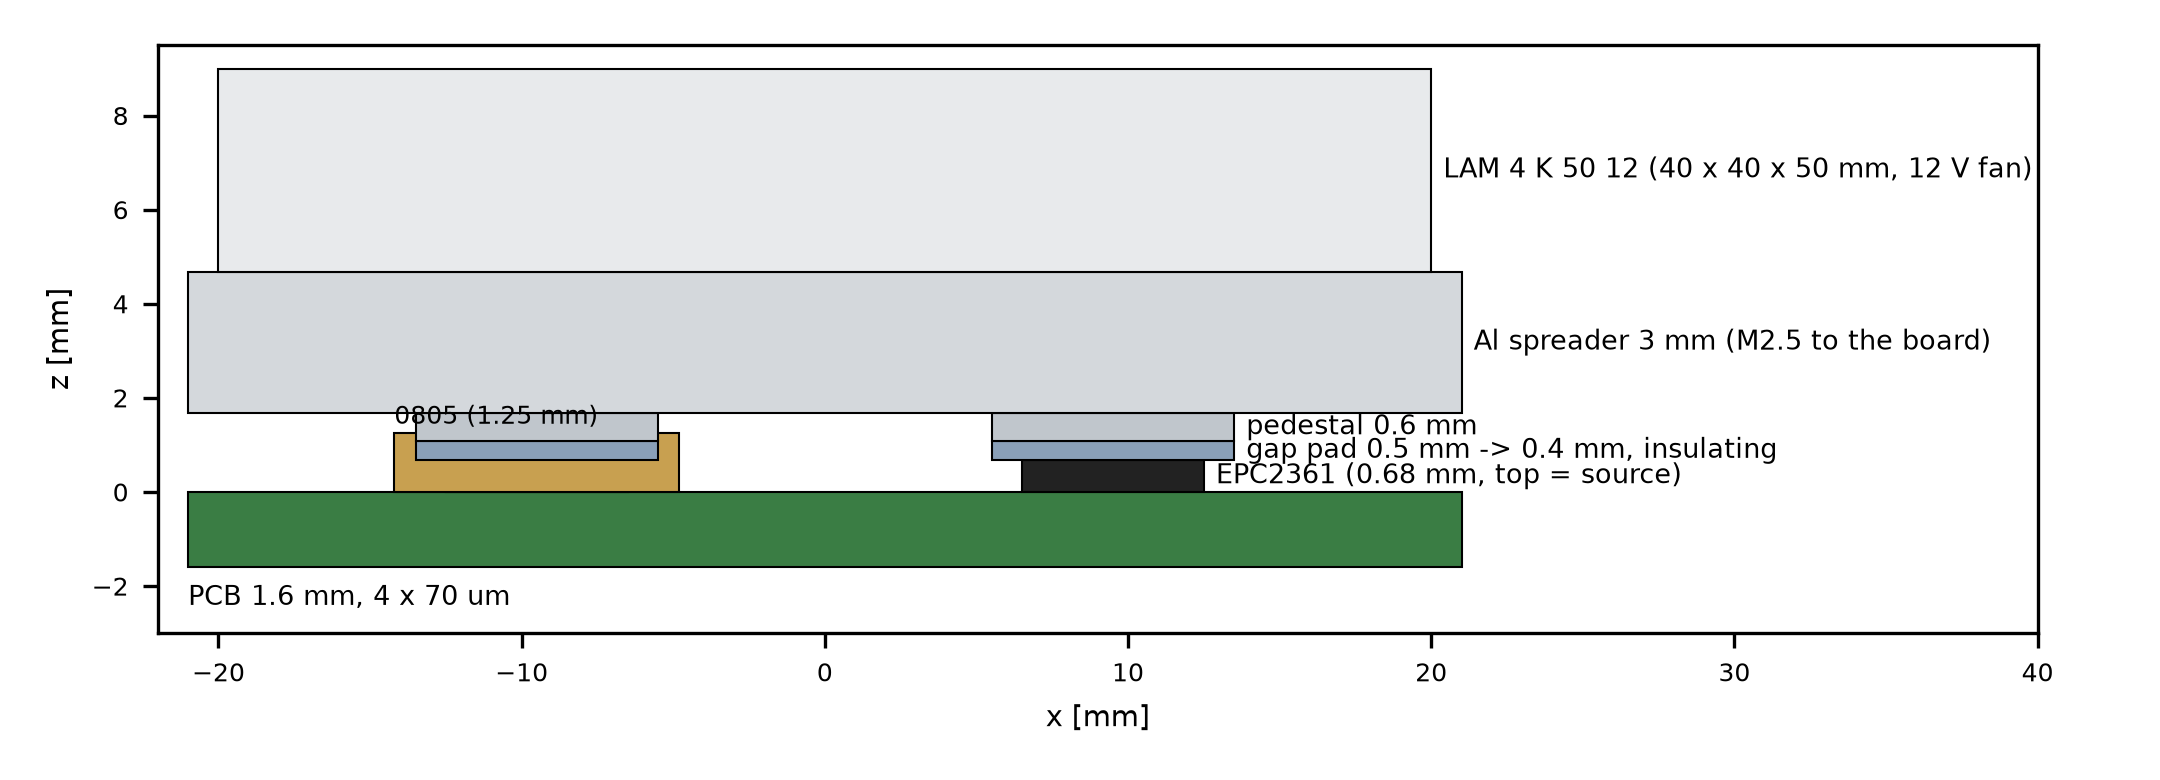
\includegraphics[width=0.9\textwidth]{fig_heatsink.png}
\caption{Thermal stack over one cell (z not to scale): EPC2361, insulating gap pad (0.5\,mm, compressed to 0.4\,mm), pedestal, spreader, Fischer LAM 4 K 50 12 with 12\,V fan. The 1210 bank capacitors (2.5\,mm) lie outside the spreader, below the heatsink base at 4.7\,mm.}
\label{fig:heatsink}
\end{figure}

\begin{table}[H]
\centering\small
\caption{Junction temperature estimate at the rated point (75\,V, 100\,A$_\mathrm{rms}$, 50\,kHz)}
\begin{tabular}{@{}lr@{}}
\toprule
Loss per transistor / in the four transistors & 1.91\,W / \PHS\,W \\
$R_{\theta\mathrm{JC}}$ (top) + gap pad (5\,W/mK, 0.4\,mm, 15\,mm$^2$) & 0.2 + \RPad\,K/W \\
Spreader + LAM 4 K 50 12 (0.65\,K/W) & \THSrise\,K rise \\
$T_j$ at 40\,$^\circ$C ambient, typical / worst-case loss & \TjHS\,/\,\TjHSWorst\,$^\circ$C \\
\bottomrule
\end{tabular}
\end{table}
The gap pad dominates: a 1\,mm pad would add about 13\,K per transistor. The pad must be insulating (the high-side tops are at the switch node, the low-side tops at DC$-$), with $\geq 1.5$\,kV breakdown for the lab and a reinforced interface in the stacked inverter. The fan is supplied from J7 (12\,V); the LAM 4 K 50 12 is a 40\,$\times$\,40\,$\times$\,50\,mm hollow profile with the fan at one end, mounted with the tube along the board so that the air flows from the tab towards the DC terminals. Proposed pad: Bergquist TGP\,5000 (Gap Pad 5000S35, 5\,W/mK, 0.020\,in = 0.51\,mm), cut to 8\,$\times$\,10\,mm, or an equivalent insulating pad of the same thickness; its breakdown rating must be checked against the 1.5\,kV requirement before ordering. The spreader is made from \texttt{fab/spb-bb-fab-spreader-drawing.pdf} (Al 6061-T6, 42\,$\times$\,13.9\,$\times$\,3\,mm plate, two 8\,$\times$\,10\,$\times$\,0.6\,mm pedestals, four M2.5 ears at $(\pm19.2,\,-7.7)$ and $(\pm19.2,\,+8.7)$\,mm, pedestals flat to 0.02\,mm, not anodised).

\section{Connectors, isolation domains and I/O}
\begin{table}[H]
\centering\small
\caption{Connectors}
\label{tab:conn}
\begin{tabularx}{\textwidth}{@{}lllX@{}}
\toprule
Ref & Part & Domain & Function \\
\midrule
J1, J2 & W\"urth REDCUBE 74650174 (THR, M4) & DC$+$, DC$-$ & submodule bus (busbar from below) \\
J3, J4 & W\"urth REDCUBE 74650174 (THR, M4) & AC (switch node) & phase output, one per cell, directly below each switch node; connect both \\
J5 & 2\,$\times$\,3 header, 2.54\,mm & primary (GNDI) & 1 +12\,V, 2 GND, 3 PWM\_H, 4 GND, 5 PWM\_L, 6 DISABLE \\
J6 & 1\,$\times$\,2 header, 2.54\,mm & LS (DC$-$) & 1 NTC (10\,k, B3380, on the low-side source copper), 2 DC$-$. \textbf{High-voltage domain}: read out only through an isolated amplifier or with the DC link discharged \\
J7 & 1\,$\times$\,2 header, 2.54\,mm & primary & heatsink fan, 1 +12\,V, 2 GND \\
TP1--TP16 & probe landings & see Tables~\ref{tab:landings}, \ref{tab:bringup} & double-pulse and bring-up measurements \\
H1--H4 / H5--H8 & M2.5 & -- & board mounting / heatsink spreader (insulated) \\
\bottomrule
\end{tabularx}
\end{table}

\begin{table}[H]
\centering\small
\caption{Minimum copper spacing between isolation domains on the routed board (pads, tracks and vias)}
\label{tab:iso}
\begin{tabular}{@{}lrr@{}}
\toprule
Domains & outer layers [mm] & inner layers [mm] \\
\midrule
DC$+$ -- HS (switch node) & \SpDcpHsOuter & \SpDcpHsInner \\
DC$+$ -- LS (DC$-$) & \SpDcpLsOuter & \SpDcpLsInner \\
HS -- LS & \SpHsLsOuter & \SpHsLsInner \\
HS -- primary & \SpHsPriOuter & \SpHsPriInner \\
LS -- primary & \SpLsPriOuter & \SpLsPriInner \\
\bottomrule
\end{tabular}
\end{table}

The power domains (DC$+$, switch node, DC$-$) differ by at most the submodule voltage (75\,V nominal, 100\,V rating) and are spaced for 100\,V under solder mask. The primary side is separated from both gate-drive domains by at least 0.8\,mm on inner and 1.37\,mm on outer layers, and by 3.35\,mm inside the 2EDF7275K package between its input and output pad rows. This is a \emph{functional} separation for a lab board with a single submodule. In the stacked 1200\,V inverter each submodule floats up to 1.2\,kV against the controller; the PWM must then arrive through reinforced isolation (fibre optics or a reinforced digital isolator on the controller side), and the 12\,V auxiliary supply must be isolated accordingly.

\section{Fabrication data and BOM}
All outputs are in \texttt{hardware/spb-bb-fab/fab/}:
\begin{itemize}\itemsep0pt
\item Gerber (L1--L4, masks, paste, silk, outline) and Gerber job file, Excellon drill file;
\item wired schematic (\texttt{spb-bb-fab.kicad\_sch}, PDF; netlist identical to the board, \texttt{scripts/check\_sch\_vs\_pcb.py}), pick-and-place (\texttt{spb-bb-fab-pos.csv}), assembly drawings top/bottom (PDF), STEP model;
\item BOM (\texttt{spb-bb-fab-bom.csv}, 35 lines, 107 placed parts, plus the mechanical and thermal items plus mounting holes and test pads).
\end{itemize}
The board is regenerated from \texttt{scripts/make\_kicad\_bb\_fab.py} (placement, power copper from the Q3D geometry, hand-placed gate loops, a domain-restricted router \texttt{scripts/fab\_router.py} for the supply and primary nets, power-via pruning, zone fill, DRC). The REDCUBE terminals are placed on the bottom side (press/solder from below); all other parts are on the top.

\begin{table}[H]
\centering\small
\caption{Main BOM items (passives in the CSV)}
\begin{tabularx}{\textwidth}{@{}rlX@{}}
\toprule
Qty & Part & Function \\
\midrule
4 & EPC2361 & power transistors \\
1 & Infineon 2EDF7275K (PG-TFLGA-13-4) & dual isolated gate driver \\
2 & Murata MGN1S1208MC-R7 & isolated 12\,V\,$\rightarrow$\,8\,V, 1\,W \\
2 & TI TPS7A4901DGNR (HVSSOP-8 PowerPAD) & 6.29\,V gate-rail regulator \\
2 & TI TLV431AIDBZR & $-1.24$\,V source-node shunt \\
12 / 24 & TDK C2012X7S2A105K125AB / Murata GRM32EC72A106KE05L & local / bank DC link \\
4 / 2 / 2 & $R_{G,i}$ 0.5\,$\Omega$ 0402 / $R_\mathrm{ON}$ 0.75\,$\Omega$ 0603 / $R_\mathrm{OFF}$ 0\,$\Omega$ 0402 & gate network (values by population) \\
2 & Nexperia PMEG3020EJ (SOD323F) & turn-off steering diodes \\
4 & W\"urth 74650174 & DC and AC terminals \\
1 & Murata NCP15XH103F03RC & NTC \\
\bottomrule
\end{tabularx}
\end{table}

\section{Verification status and checklist}
\begin{table}[H]
\centering\small
\begin{tabularx}{\textwidth}{@{}lX@{}}
\toprule
Done & DRC (0 violations, 0 unconnected); schematic netlist identical to the board (239 pins, \texttt{scripts/check\_sch\_vs\_pcb.py}); domain spacing (Table~\ref{tab:iso}); gate budget and peak currents (Table~\ref{tab:budget}); footprints of the 2EDF7275K (datasheet Fig.~22) and MGN1 (KDC\_MGN1 p.~17) entered from the datasheets; EPC land pattern from EPC. \\
Open, before ordering & Q3D extraction of the routed copper (prepared, needs the licence server); footprint review of the custom LGA and MGN1 pads against the latest drawings; fab-house review of the 0.2\,mm power gaps and the 0.45/0.25\,mm Kelvin vias; thermal check of the AC path (two terminals, 4 layers 2\,oz). \\
Bring-up & Power-up order: 12\,V first, DC link last; power-down in reverse (R41/R42 hold the gates off when the driver side is unpowered, but do not replace the order). (1) 12\,V only, 20\,mA current limit: D7, D3--D6 on; TP9--TP14 per Table~\ref{tab:bringup}. (2) PWM on J5 without DC link: OUT and gate waveforms on R5/R7 and R1--R4, dead time from the controller. (3) Double-pulse test at 12, 24, 48, 75\,V with an external bulk capacitor ($\geq$\,1\,mF) on J1/J2: $V_\mathrm{DS}$ (TP1/TP5), $V_\mathrm{GS}$ (TP3/TP7), $v_\mathrm{KS}$ (TP2/TP6), inductor current with a Rogowski coil; compare $E_\mathrm{on}$, $E_\mathrm{off}$ and the high-side bump (TP4/TP8, isolated probe) with the simulation. (4) Heatsink, continuous operation, thermal camera on the outer edges. \\
\bottomrule
\end{tabularx}
\end{table}

\end{document}
